\chapter{ĐÁNH GIÁ KẾT QUẢ}
Trong chương này, chúng tôi sẽ trình bày chi tiết về các kết quả đạt được trong quá trình triển khai thực hiện đề tài, từ đó đưa ra những kết luận về những thành tựu đạt được, cũng như những thách thức và hạn chế gặp phải trong quá trình thực hiện. Các kết quả đạt được của đề tài sẽ cung cấp cho chúng ta một cái nhìn tổng quan về tiềm năng, tính hiệu quả, khả năng mở rộng và ứng dụng vào thực tế của việc điều khiển và giao tiếp thiết bị dựa trên OPC-UA. 

\section{Kết quả đạt được}
\subsection{Control}
Module Control là module quan trọng trọng trong kiến trúc hệ thống, là nơi tiếp nhận tín hiệu điều khiển và cập nhật trạng thái của cánh tay lên OPC, tại đây nhóm đã hiện thực thành công 2 thành phần quan trọng của module Control đó là một Server OPC giao tiếp với Datacenter và một chương trình điều khiển cánh tay Jetmax cùng với các chức năng AI kèm theo.
\begin{itemize}
    \item Server OPC: Ở server OPC nhóm đã hiện thực thành công một server OPC đơn giản chứa các node dữ liệu của cánh tay ( tọa độ, tốc độ, gốc servo, trạng thái AI,...) và các method phục vụ cho việc điều khiển cánh tay. Các method này sẽ gọi tới các ROS service được hiện thực trong chương trình điều khiển cánh tay. Ngoài ra giao tiếp giữa Server và Datacenter được nhóm thực hiện mã hóa thông qua các certificate mà nhóm tự generate, nhầm đảm an toàn cho dữ liệu trong qua trình giao tiếp giữa 2 module thông qua OPC. Dưới đây là hình ảnh cấu trúc thư mục của server opc và ảnh các gói tin được mã hóa trên phần mềm Wireshark:
    \begin{figure}[H]
    \centering
    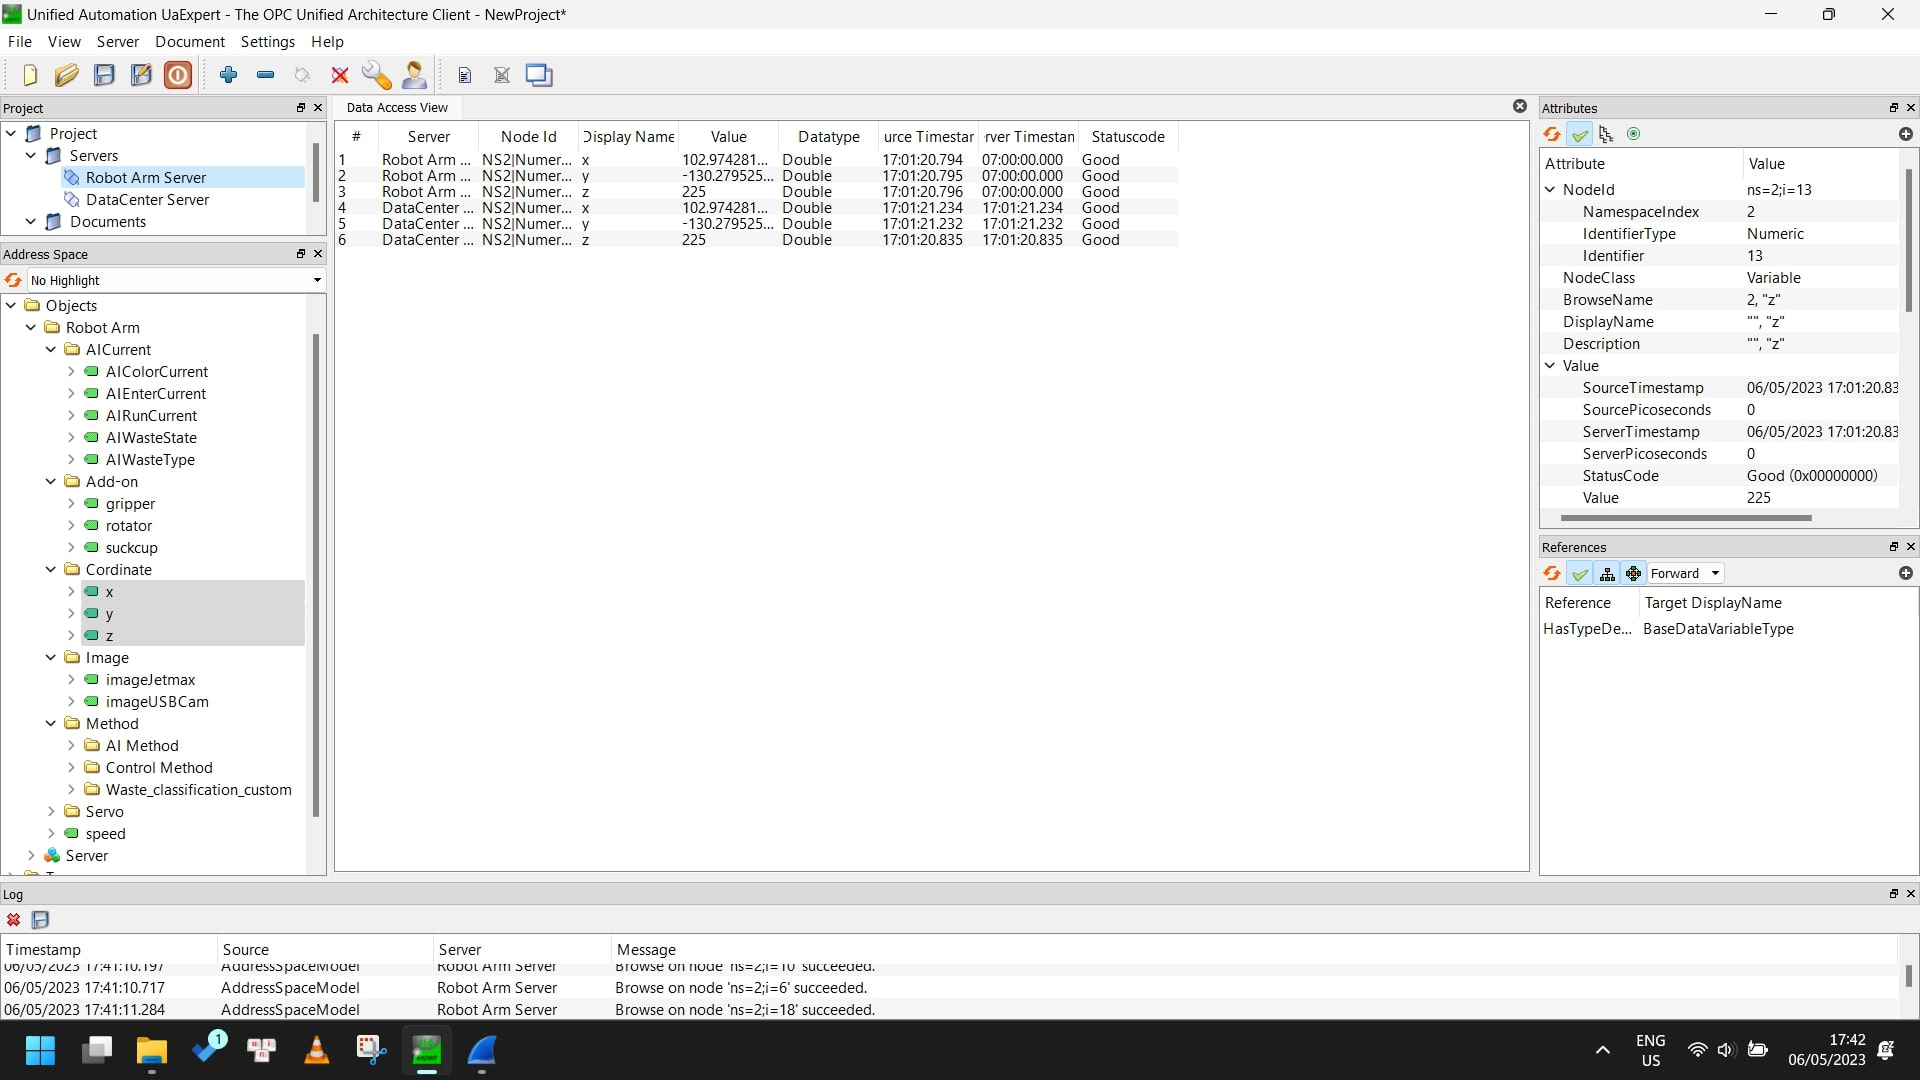
\includegraphics[width=0.9\textwidth]{Images/Result/datastructure_server.jpg}
    \caption{Cấu trúc thư mục của server opc}
    \end{figure}
    
    \begin{figure}[H]
    \centering
    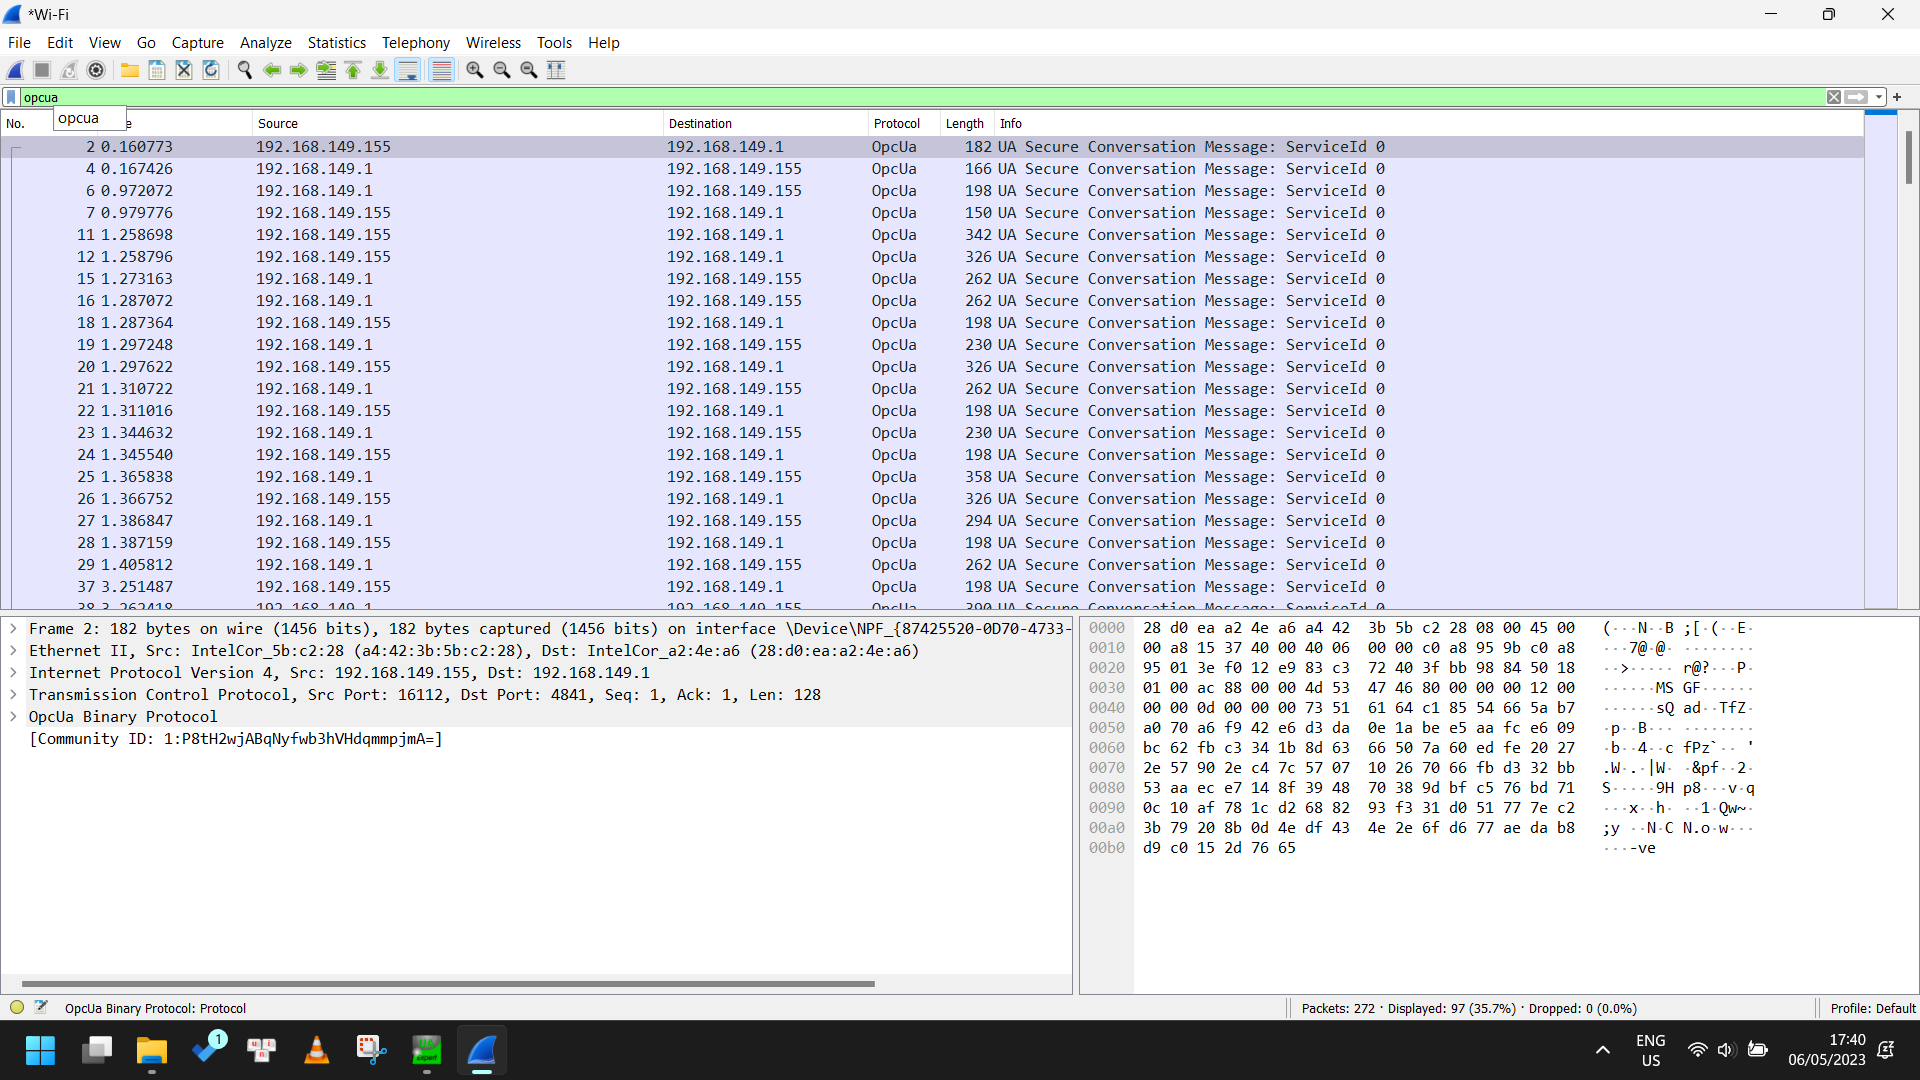
\includegraphics[width=0.9\textwidth]{Images/Result/wireshark.png}
    \caption{Hình ảnh gói tin trên Wireshark}
    \end{figure} 
    
    \item Chương trình điều khiển cánh tay và chức năng AI: Ngoài những AI đã được tích hợp trong cánh tay Jetmax, nhóm đã hiện thực thành công một tính năng AI mới với chức năng phân loại rác bán tự động, ở mô hình AI này nhóm đã kết hợp sử dụng 2 thư viện nổi tiếng đó là OpenCv và Yolov5. Với Yolov5 nhóm sử dụng để nhận diện các vật thể đã được training trước đó thông qua phương pháp học máy suppervise learning, với OpenCV nhóm sử dụng để nhận diện các thùng chứa những loại rác tương ứng qua các màu sắc của nó. Tuy nhiên, mô hình sẽ không hoàn thiện và chức năng sẽ không ổn định nếu thiếu đi bước tính toán tìm vị trí của vật thể đó so với tọa độ của cánh tay. Bên dưới đây là một số hình ảnh về kết quả đạt được ở chức năng AI này.
    
    \begin{figure}[H]
    \centering
    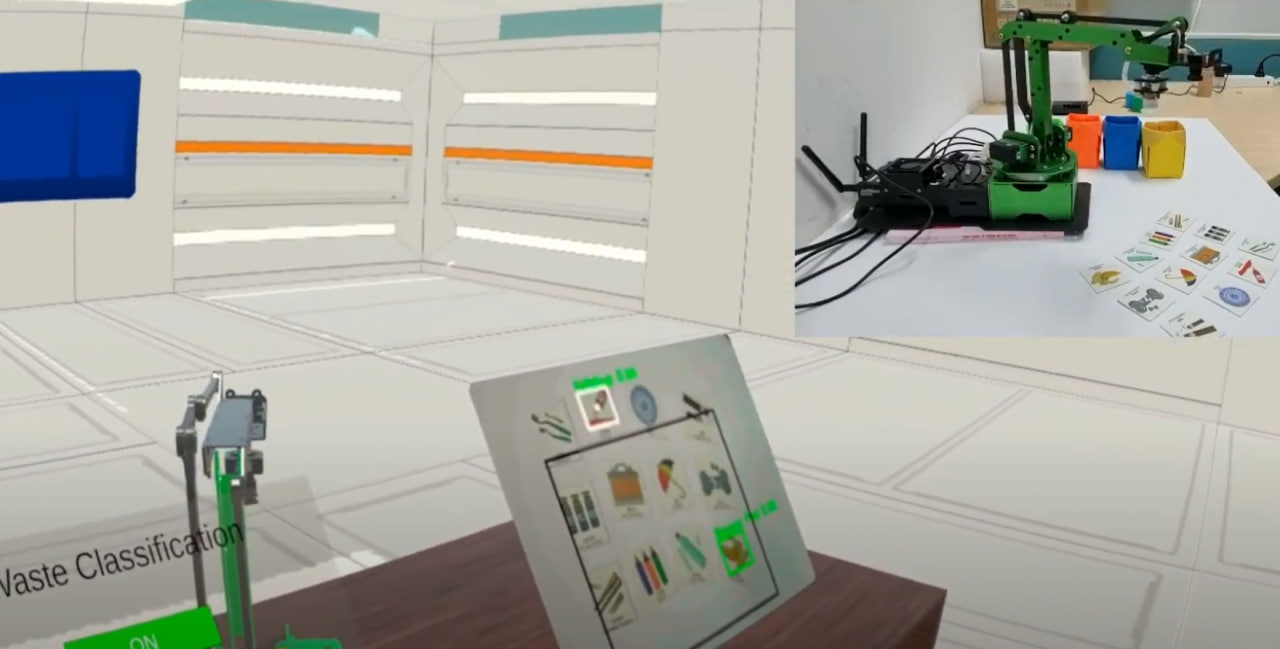
\includegraphics[width=0.9\textwidth]{Images/Result/ai-result-1.jpg}
    \caption{Nhận diện rác và hiển thị lable}
    \end{figure}
    
    \begin{figure}[H]
    \centering
    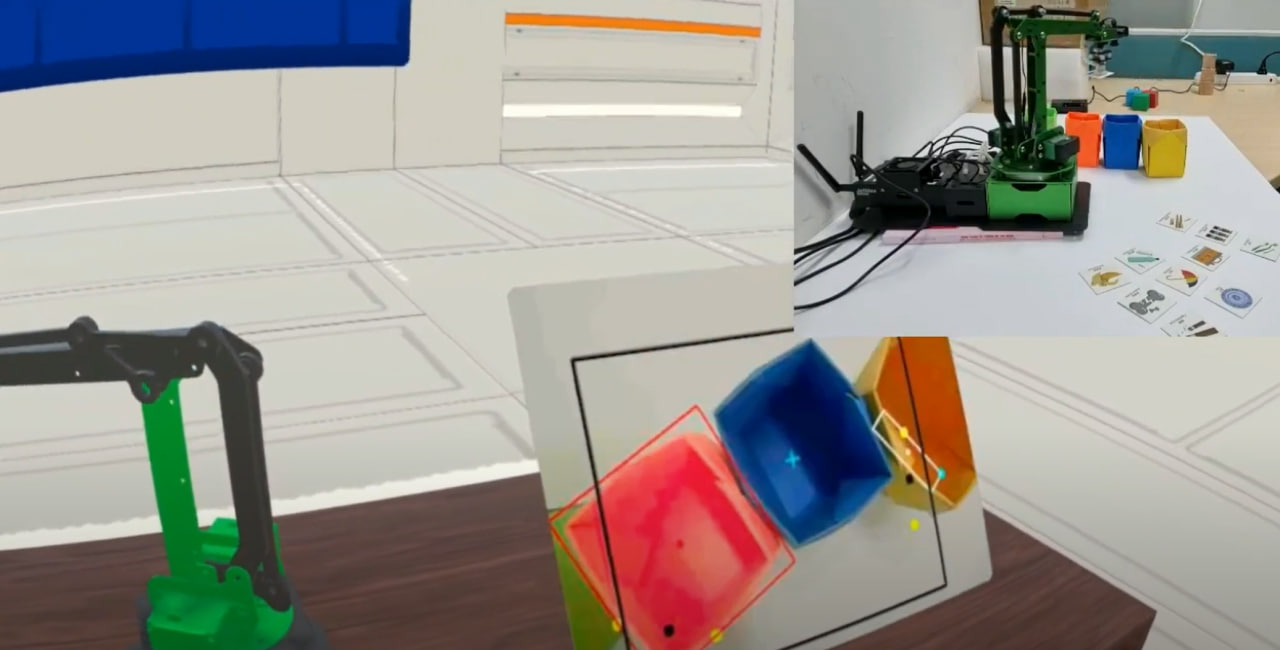
\includegraphics[width=0.9\textwidth]{Images/Result/ai-result-2.jpg}
    \caption{Nhận diện thùng rác qua màu sắc}
    \end{figure} 
\end{itemize}



\subsection{DataCenter}

Đối với Datacenter, nhóm đã hiện thực thành công theo kiến trúc đã đề xuất. Datacenter gồm một sub-client OPC UA kết nối với OPC UA server trên module Control, thu thập cấu trúc dữ liệu node và tạo các bản sao cùng chức năng lên sub-server OPC UA. Datacenter cũng có khả năng tự hồi phục khi kết nối tới server OPC UA bị ngắt: Datacenter khi đó sẽ hủy toàn bộ thông tin node bản sao, cố kết nối lại sau mỗi 2 giây và khi thành công, tạo mới lại cấu trúc node khi kết nối được phục hồi. Hiện tại, Datacenter của nhóm đã có thể "sao chép" cấu trúc node tương tự như cấu trúc node OPC UA server trên module control, với các node variable sẽ liên tục cập nhật dữ liệu, còn các node method sẽ hoạt động như một "wrapper" và gọi đến method gốc trên module Control. Chương trình Datacenter được lập trình sử dụng python, tận dụng thư viện asyncua - một thư viện nâng cấp so với FreeOpcUa, với hiệu năng tốt hơn, code được viết dễ quản lý hơn nhờ tận dụng cú pháp của các hàm async trong Python. Tuy nhiên, Datacenter chỉ có thể tạo bản sao của các kiểu node biến (variable), node thư mục (folder) và node hàm (method) và chưa thể tạo bản sao của các cấu trúc node dạng object phức tạp hay do người dùng tự định nghĩa.

Dưới đây là hình ảnh cấu trúc node của Datacenter giống hệt cấu trúc node trên module Control, và các giá trị node variable cũng tương tự.

    \begin{figure}[H]
    \centering
    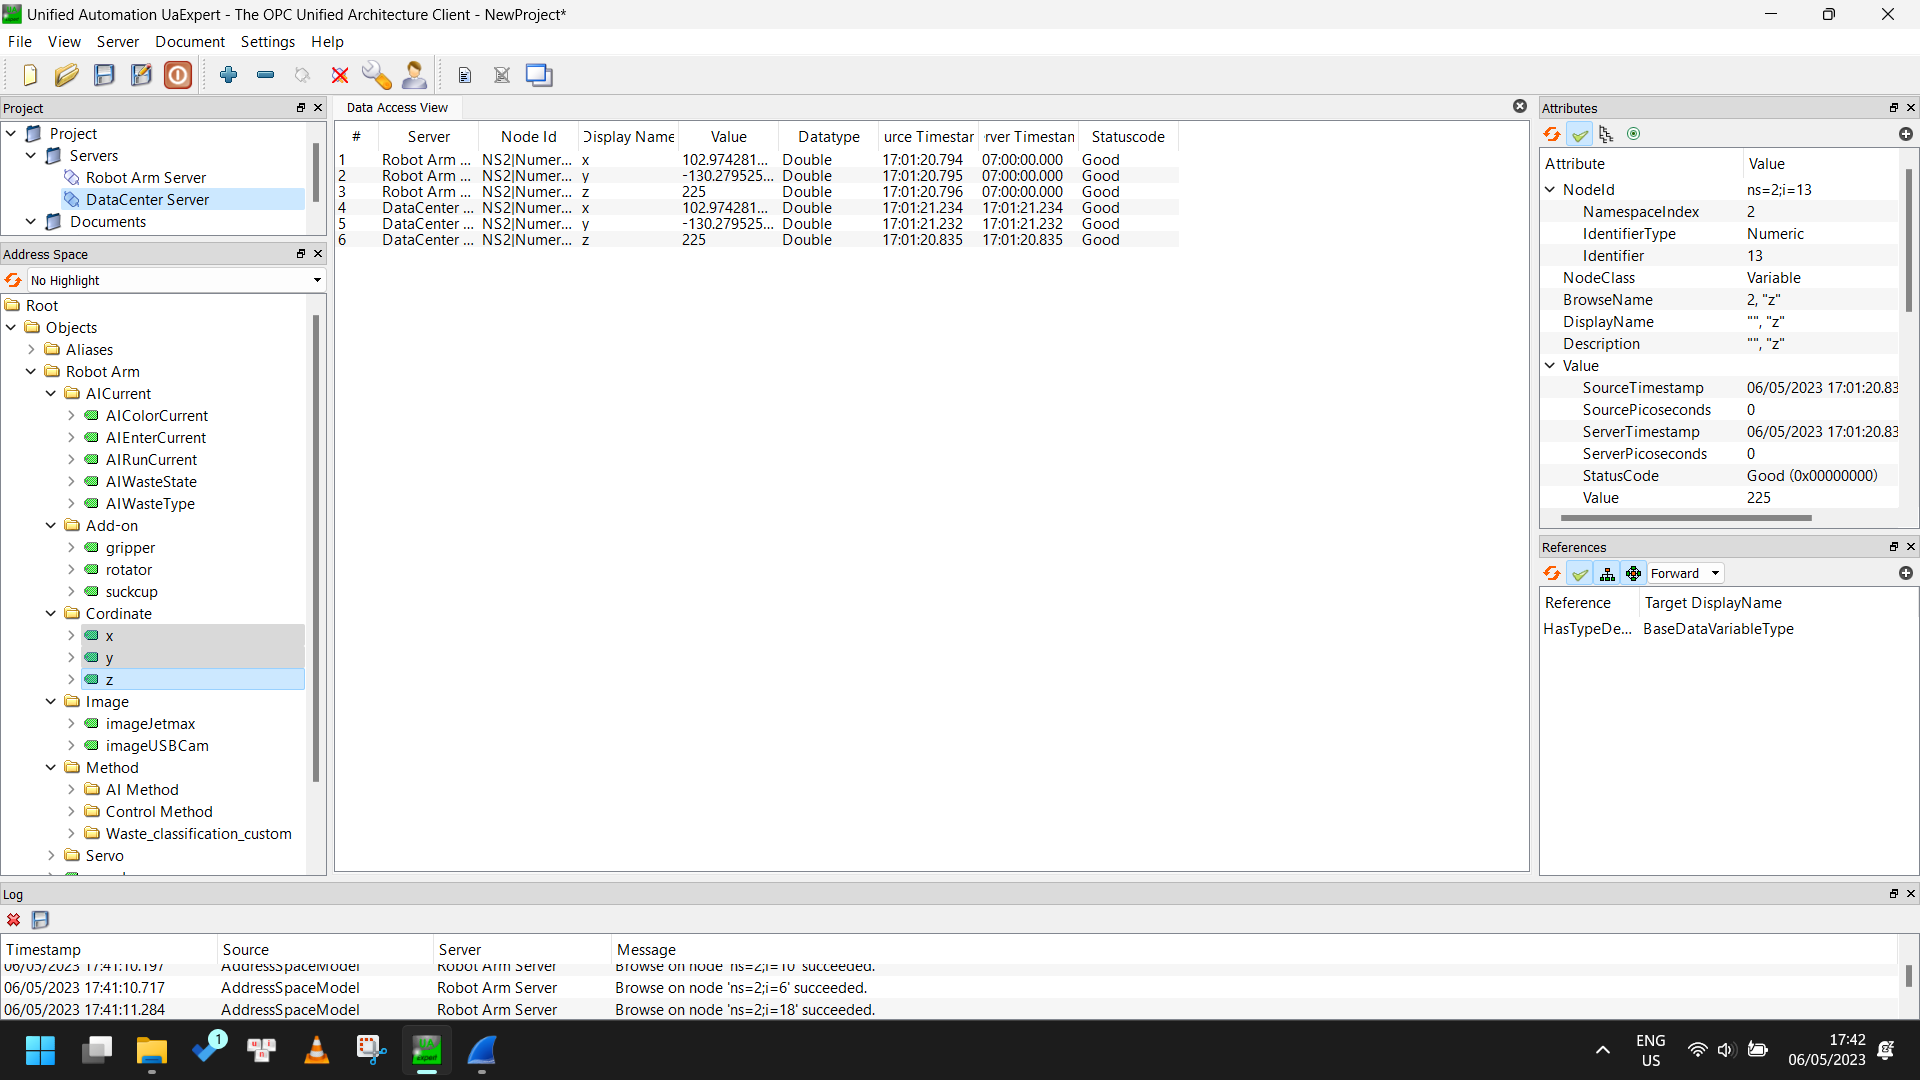
\includegraphics[width=0.9\textwidth]{Images/Result/opc-structure_data.png}
    \caption{Cấu trúc thư mục của Datacenter giống hệt với module Control}
    \end{figure}


\subsection{VR Application}

Ứng dụng VR được nhóm thực hiện như một ứng dụng digital twin nhằm điều khiển cánh tay robot Jetmax. Ứng dụng này cũng chính là một OPC UA client có thể kết nối tới OPC UA server trên Datacenter nhằm thu thập dữ liệu và gửi lệnh điều khiển. Ứng dụng được phát triển sử dụng Unity, sinh ra file apk và nạp, sử dụng trên kính Oculus Quest 2. Khi vào ứng dụng, ta sẽ thấy được khung cảnh VR, mô hình 3D của cánh tay, một của sổ để Debug và một bảng menu để điều khiển. Nếu bảng điều khiển menu quá cao/thấp hoặc to, người dùng có thể nắm khối đen hình trụ ngang để thay đổi vị trí, hoặc dùng hai tay nắm khối trụ để phóng to/thu nhỏ bảng điều khiển. 

\begin{figure}[H]
    \centering
    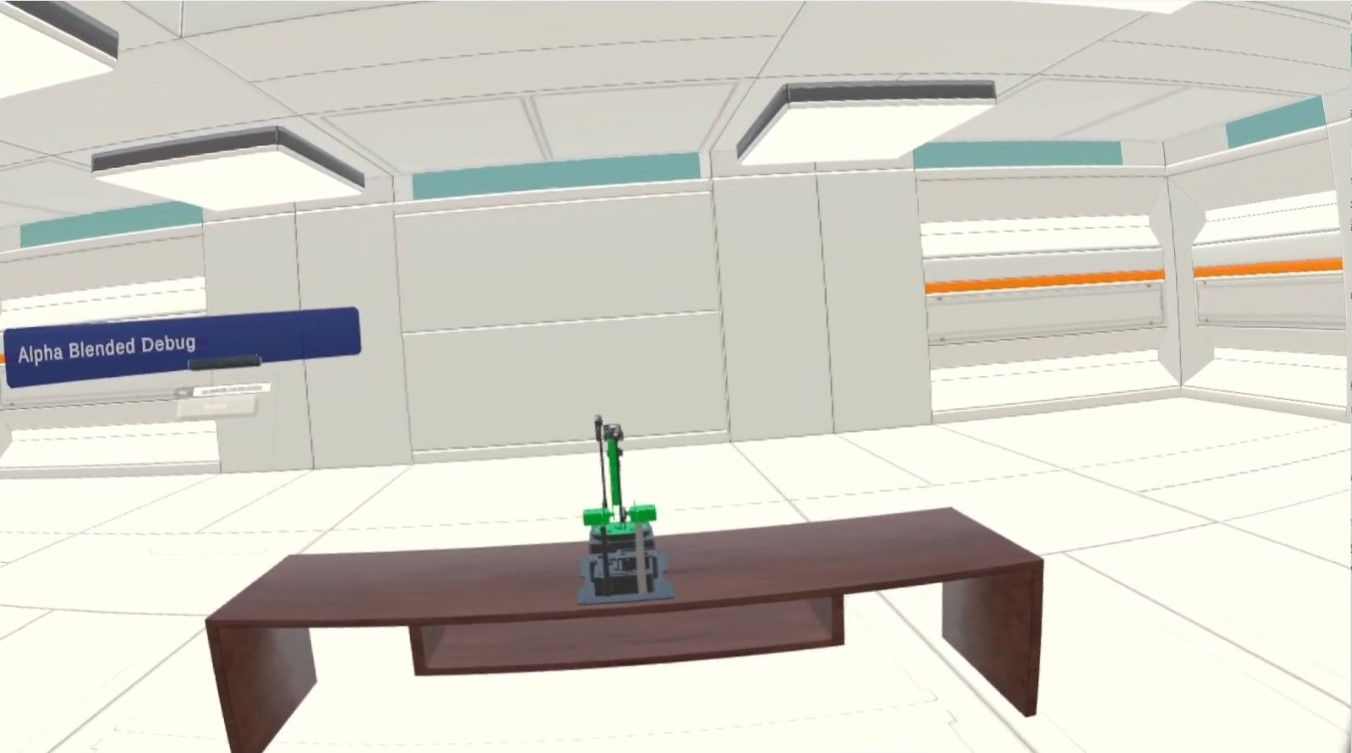
\includegraphics[width=0.9\textwidth]{Images/Result/vr_foreground.jpg}
    \caption{Giao diện ứng dụng khi vừa khởi động}
    \label{fig:vr_foreground}
\end{figure}

Trên bảng điều khiển, người dùng có thể nhấn chạm vào khung URL để nhập địa chỉ OPC UA server cần kết nối tới, và bấm nút Connect để tiến hành kết nối. Giao diện ứng dụng sẽ thay đổi để bảo cho người dùng về trạng thái kết nối. Nếu kết nối thất bại, màn hình debug sẽ hiện ra lỗi và stacktrace của lỗi, ngược lại, kết nối thành công sẽ hiện toàn bộ khung menu với vô số các nút nhấn điều khiển như GoHome, Increase Speed, Decrease Speed, đồng thời cho phép người dùng sử dụng các nút bấm trên tay cầm để điều khiển hoạt động của cánh tay một cách thủ công. Thêm nữa, người dùng có thể nhấn nút Disable Controller để tắt khả năng điều khiển cánh tay bằng tay cầm, thực hiện thao tác khác như điều chỉnh vị trí và kích cỡ menu. Khi cảm thấy thoải mái, người dùng có thể quay trở lại điều khiển bằng cách nhấn nút Enable controller. Và quan trọng nhất, ở trạng thái kết nối, mô hình 3D của cánh tay sẽ phản ánh trạng thái thực tế của cánh tay -  thông qua việc OPC UA client trên ứng dụng liên tục thu thập dữ liệu góc xoay của cánh tay thực tế. Hoạt động của cánh tay 3D trong môi trường VR đem lại cảm giác điều khiển chân thực và thú vị hơn cho người dùng.

\begin{figure}[H]
    \centering
    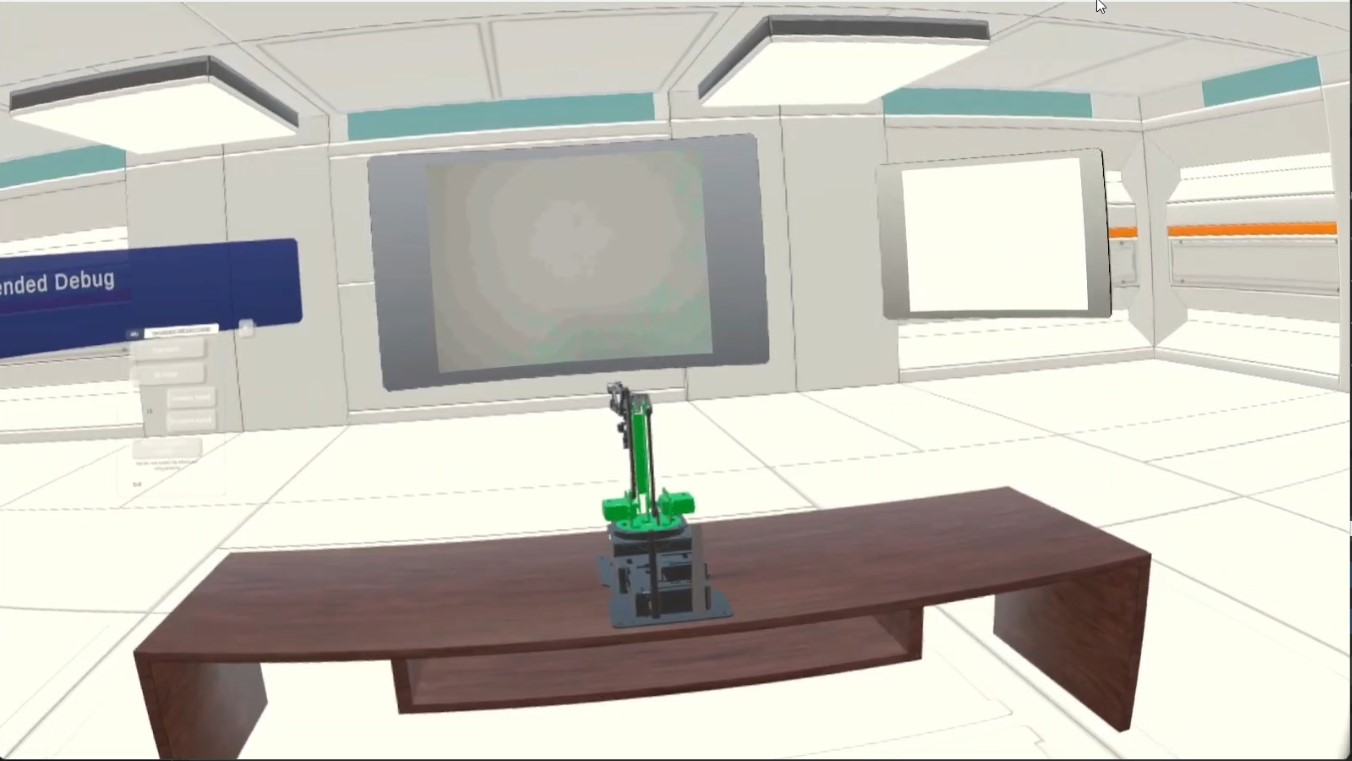
\includegraphics[width=0.9\textwidth]{Images/Result/vr_success.jpg}
    \caption{Giao diện ứng dụng kết nối thành công}
    \label{fig:vr_success}
\end{figure}

\begin{figure}[H]
    \centering
    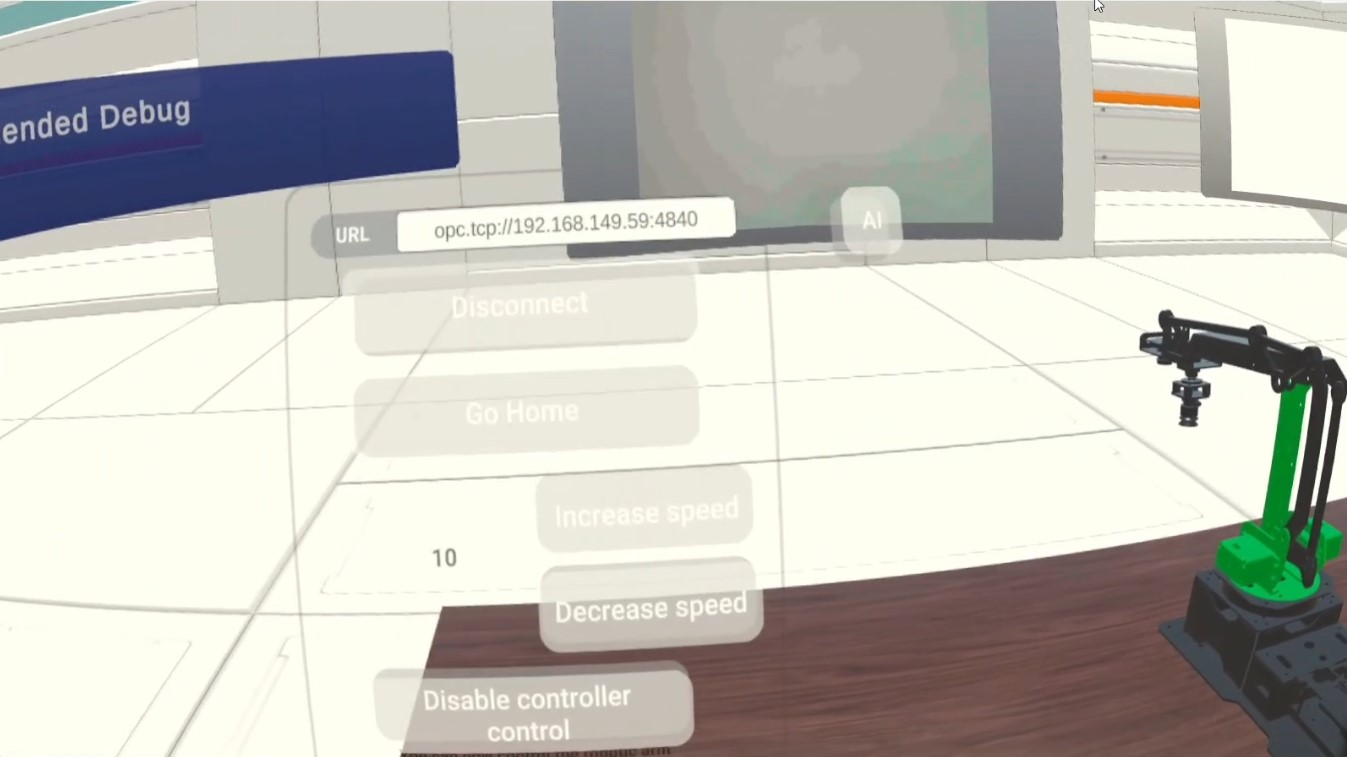
\includegraphics[width=0.9\textwidth]{Images/Result/vr_menu.jpg}
    \caption{Bảng menu điều khiển}
    \label{fig:vr_menu}
\end{figure}

Không chỉ thế, ứng dụng còn cung cấp cho người dùng khả năng kích hoạt, sử dụng 3 chức năng AI: Phân loại rác bán tự động, theo dõi khối màu và xếp gỗ. Trong suốt thời gian sử dụng các tính năng AI, trạng thái cánh tay thực vẫn sẽ luôn cập nhật lên mô hình 3D của cánh tay trong không gian VR nhanh chóng và trực quan. Người dùng cần nhấn nút "AI" kế bên menu để mở bảng điều khiển AI. Tiếp theo, ta sẽ quan sát bảng điều khiển của từng chức năng AI cụ thể

\begin{figure}[H]
    \centering
    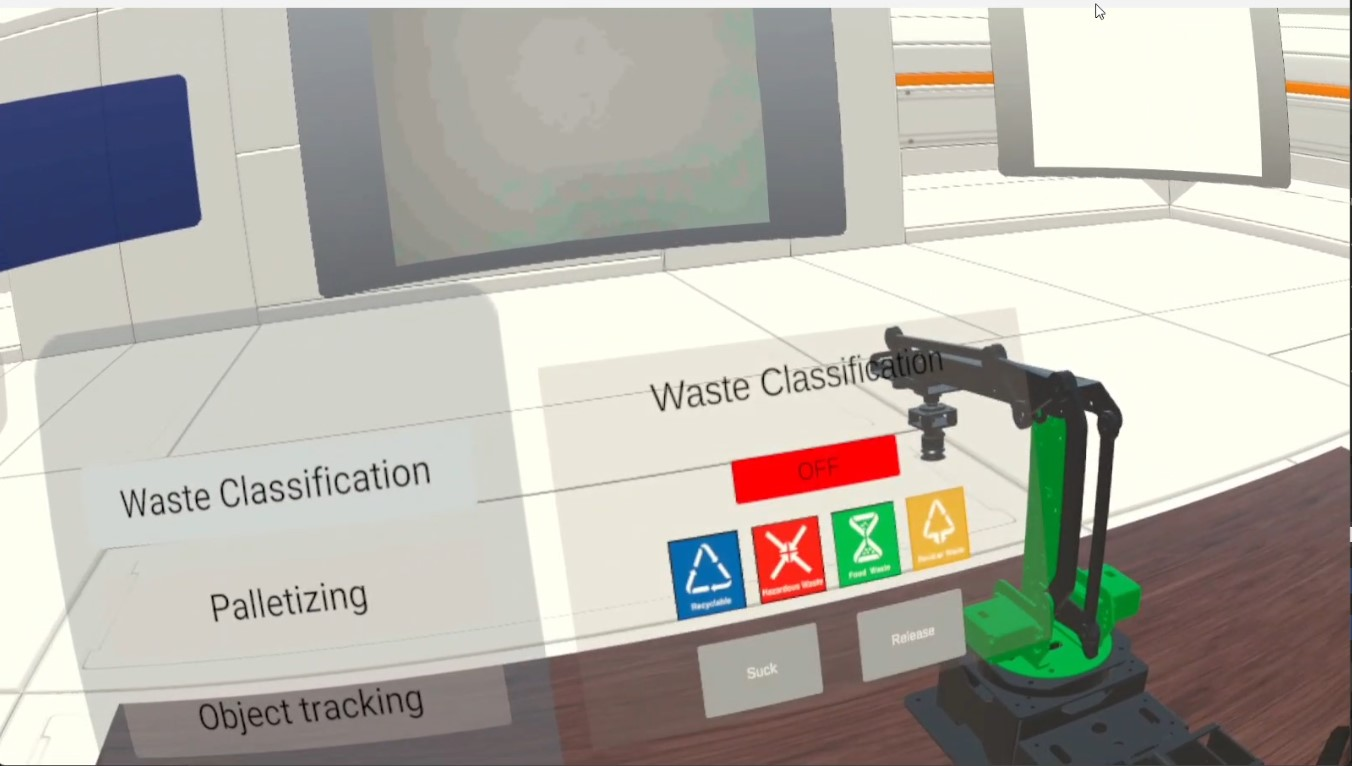
\includegraphics[width=0.9\textwidth]{Images/Result/vr_waste.jpg}
    \caption{Giao diện AI phân loại rác bán tự động}
    \label{fig:vr_waste}
\end{figure}

Người dùng nhấn vào "Waste Classification" để mở bảng điều khiển cho Phân loại rác bán tự động. Mặc định, chức năng sẽ bắt đầu nhận diện loại rác thải đồ ăn (Food Waste), và người dùng có thể chọn các loại rác khác như rác nguy hiểm (Hazardous waste), rác có thể tái chế (Recycable Waste) và rác thải đô thị (Residual Waste), tuy nhiên chỉ có thể chọn một trong bốn loại rác. Người dùng nhấn vào nút "ON" để bắt đầu chạy AI. Khi này, chương trình AI Phân loại rác sẽ vào trạng thái 1: IDLE, camera sẽ thu hình ảnh và nhận diện loại rác. Người dùng cần điều khiển cánh tay thủ công tới khu vực có rác và nằm trong khối vuông trên camera. Khi camera đã nhận diện được, người dùng có thể nhấn nút "Suck" để cánh tay tự động hút rác lên. Khi hút thành công, người dùng cần điều khiển thủ công cánh tay tới khu vực thùng rác và để camera tự nhận diện thùng rác đúng loại rác đã chọn. Nhấn nút "Release", cánh tay sẽ tự động thả rác xuống thùng rác phù hợp, và quay về trạng thái IDLE, sẵn sàng để phân loại rác tiếp theo.

\begin{figure}[H]
    \centering
    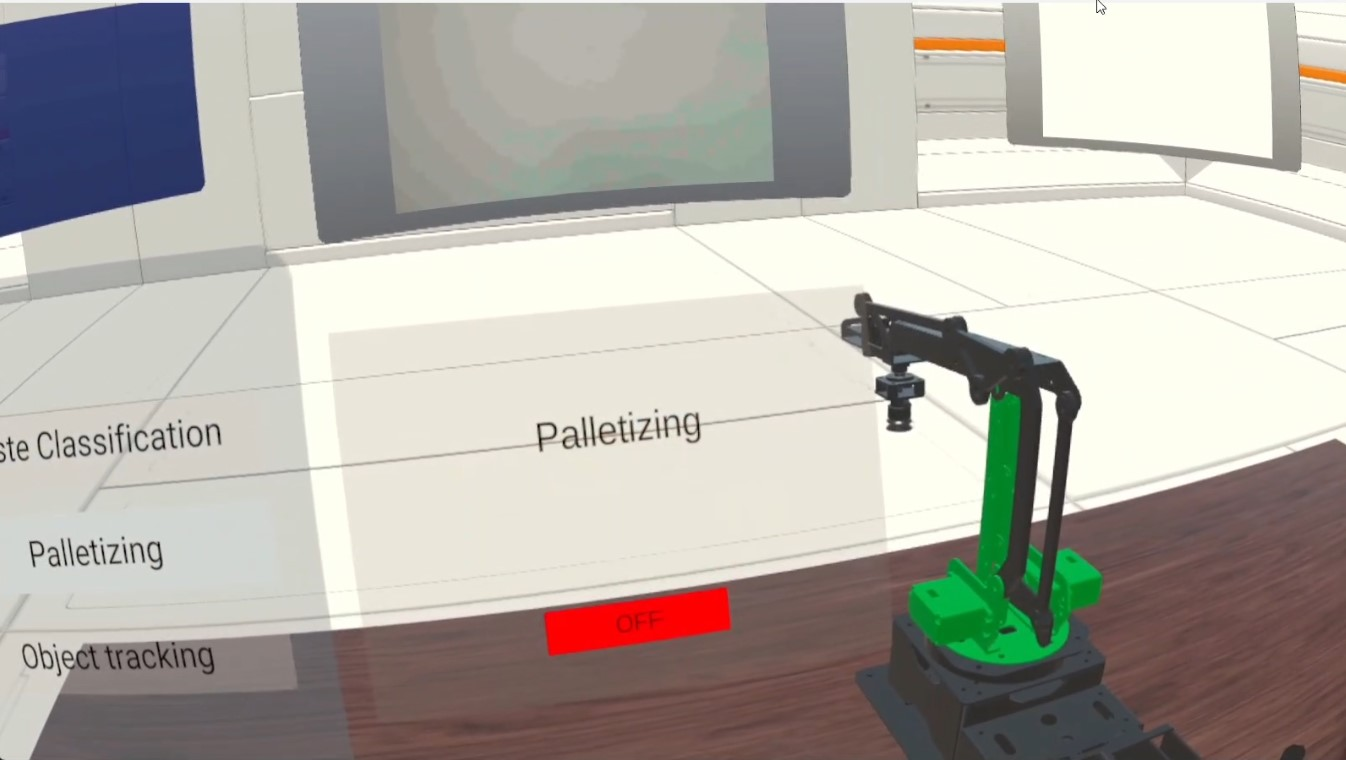
\includegraphics[width=0.9\textwidth]{Images/Result/vr_blocks.jpg}
    \caption{Giao diện AI xếp chồng khối gỗ}
    \label{fig:vr_blocks}
\end{figure}

Đây là một chức năng AI thú vị được cung cấp sẵn bởi nhà sản xuất Hiwonder. Khi người dùng bấm kích hoạt chức năng này và bản điều khiển hiện ra, cánh tay sẽ quay về vị trí ban đầu. Người dùng cần đặt ba khối gỗ có mặt code QR hướng lên camera để nhận diện. Sau đó, nhấn nút "ON". Cánh tay sẽ ngay lập tức nhận diện ba khối gỗ và lần lượt xếp chồng chúng lên nhau tại một vị trí đã được lập trình trước đó. Chức năng này vẫn còn yếu điểm là không thể nhận biết được đã xếp bao nhiêu khối, chỉ biết sắp xếp theo thứ tự khối 1, 2, 3 với độ cao tăng dần rồi vòng về lại, và đôi khi sẽ thả quá cao hoặc quá thấp.

\begin{figure}[H]
    \centering
    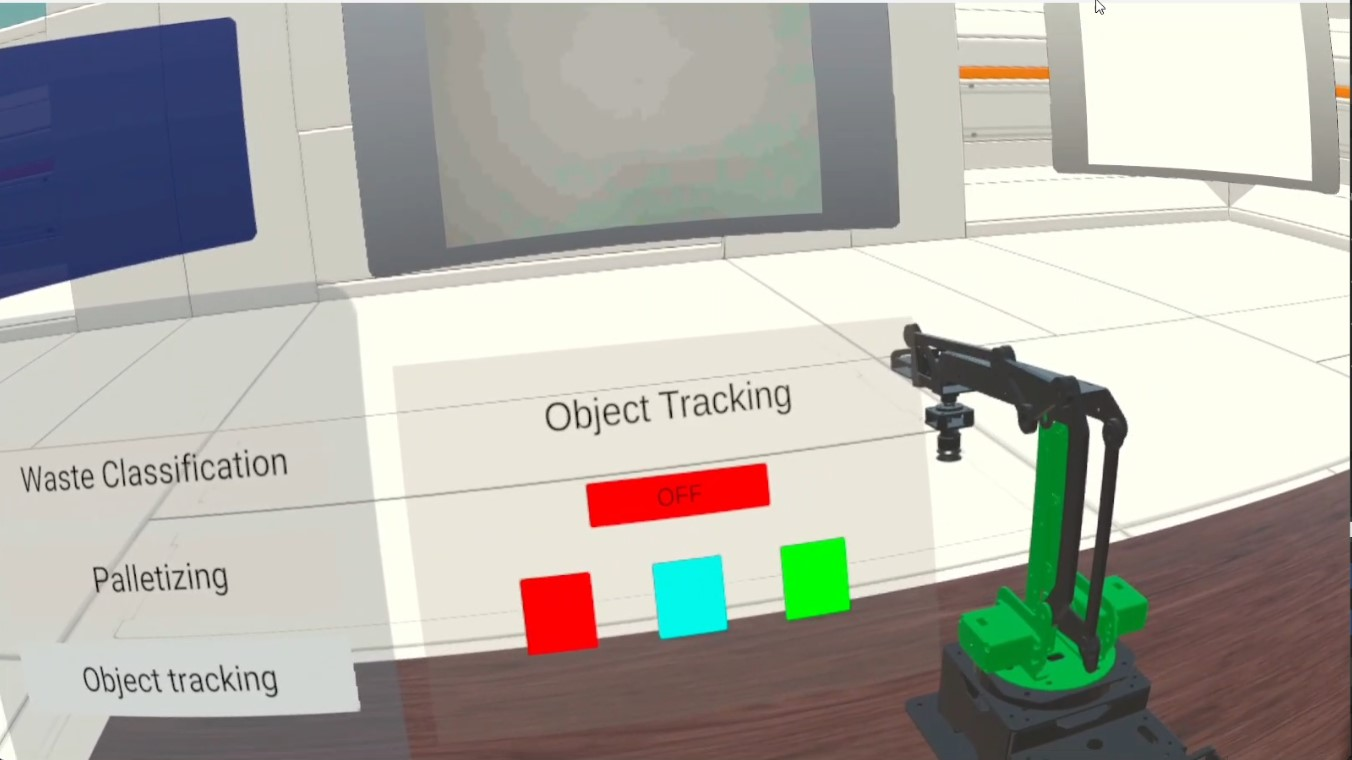
\includegraphics[width=0.9\textwidth]{Images/Result/vr_color_tracking.jpg}
    \caption{Giao diện AI theo dõi khối màu}
    \label{fig:vr_color_tracking}
\end{figure}

Đây cũng là một chức năng cung cấp sẵn bởi nhà sản xuất Hiwonder. Khi kích hoạt tính năng, cánh tay sẽ quay về vị trí mặc định. Người dùng chạy tính năng bằng cách nhấn nút "ON", sau đó chọn một trong 3 màu đỏ - xanh lá - xanh dương để theo dõi. Khi đặt vật thể thực tế trùng với màu đã chọn, cánh tay sẽ di chuyển theo vị trí của khối màu, và sự chuyển động này cũng được thể hiện trực quan trên mô hình 3D của ứng dụng VR.

Nhóm mong đợi rằng việc điều khiển được cánh tay trong môi trường VR sẽ đem lại trải nghiệm điều khiển chân thực hơn cho người dùng, và có thể mở rộng trong môi trường công nghiệp, với tình huống khi người quản trị cần điều khiển cánh tay robot để thực hiện các thao tác nguy hiểm, hoặc người quản trị muốn điều khiển cánh tay từ xa để xử lý vấn đề mà không cần có mặt trực tiếp. Giao thức OPC UA được sử dụng cho giao tiếp giữa ứng dụng và trung tâm dữ liệu đảm bảo cho sự an toàn, bảo mật của thông tin cũng như tốc độ, độ ổn định của dữ liệu giao tiếp, giúp thao tác điều khiển chính xác, hiệu quả hơn.

Video demo cho hệ thống của nhóm có thể xem ở đây: \href{https://drive.google.com/drive/folders/19mNmhoP1a_-qYdjnaqDzg5lH_5AGWdpT?usp=sharing}{https://drive.google.com/\\drive/folders/19mNmhoP1a\_-qYdjnaqDzg5lH\_5AGWdpT?usp=sharing}


\section{Kiểm tra đánh giá hệ thống}

Ở phần này, nhóm sẽ thực hiện một số thử nghiệm để đánh giá hoạt động và khả năng của hệ thống. Ở phần thử nghiệm đầu tiên, nhóm sẽ đánh giá về mức độ sử dụng CPU của module Server và module Datacenter; mức độ sử dụng CPU, GPU và số lượng khung ảnh trên giây (Frame per second - fps) của ứng dụng trên kính Oculus; thời gian xoay vòng (Round Trip Time) của hệ thống trong kiến trúc được đề xuất. Phần thứ hai, nhóm sẽ đánh giá độ chỉnh xác của giải thuật điều khiển cánh tay Phân loại rác và thả rác vào thùng cùng với khả năng nhận diện rác thải trong chức năng phân loại rác bán tự động mà nhóm phát triển.

\subsection{Đánh giá hoạt động hệ thống}

Để có những đánh giá về hoạt động của hệ thống, nhóm thực hiện ba thí nghiệm trong điều kiện khác nhau, mỗi thí nghiệm sẽ thực hiện ra lệnh điều khiển thiết bị từ ứng dụng trên kính oculus 100 lần, từ đó đo đạc thông số hoạt động của các module trong kiến trúc hệ thống. Ba điều kiện thí nghiệm được đề ra như sau:

\begin{itemize}
    \item Chỉ có ứng dụng kết nối với Datacenter
    \item Có 5 client và ứng dụng kết nối với Datacenter
    \item Có 10 client và ứng dụng kết nối với Datacenter
\end{itemize}

Việc thực hiện thí nghiệm như trên cũng giúp nhóm đánh giá khả năng chịu tải của Datacenter khi có lượng lớn mini-client kết nối và điều khiển thiết bị trong tương lai. Các client được chạy trên Laptop chung mạng với các thiết bị, và các client kết nối thêm vào Datacenter này sẽ luôn đọc dữ liệu toàn bộ các node variable chứ không tham gia vào quá trình điều khiển. Cấu hình của các thiết bị trong thí nghiệm này như sau:

\begin{itemize}
    \item Module Control: Jetson Nano B01
    \begin{itemize}
        \item 128-core Maxwell GPU
        \item Bộ xử lý A57 lõi tứ với 1.43GHz
        \item Bộ nhớ hệ thống: 4GB 64-bit LPDDR4 với tốc độ 25.6GB/s
    \end{itemize}
    \item Module Datacenter: Raspberry Pi 4 model B
    \begin{itemize}
        \item Boardcom VideoCore VI GPU
        \item Bộ xử lý Cortex-A72 (ARM v8) 64-bit SoC với 1.5GHz
        \item Bộ nhớ 4GB LPDDR4-2400MHz
    \end{itemize}
    \item Module VR app: Oculus Quest 2
    \begin{itemize}
        \item Chipset Qualcomm Snapdragon XR2
        \item Adreno 650 GPU
        \item Bộ xử lý lõi bát Kryo 585 (1 x 2.84 GHz, 3 x 2.42 GHz, 4 x 1.8 GHz)
        \item Bộ nhớ 6GB
    \end{itemize}
    \item Các Mini-client: Laptop Dell Inspiron 3501
    \begin{itemize}
        \item NVIDIA MX330 GPU
        \item Bộ xử lý lõi tứ Intel i5-1135G7 với 2.40GHz
        \item Bộ nhớ 16GB LPDDR4-3200MHz
    \end{itemize}
\end{itemize}

\subsubsection{Đánh giá Module Control}

Thực hiện ba thí nghiệm trên, nhóm thực hiện đo đạc mức độ sử dụng CPU và lượng RAM sử dụng của chương trình server OPC trên module control, cho ra được biểu đồ sau:

\begin{figure}[H]
    \centering
    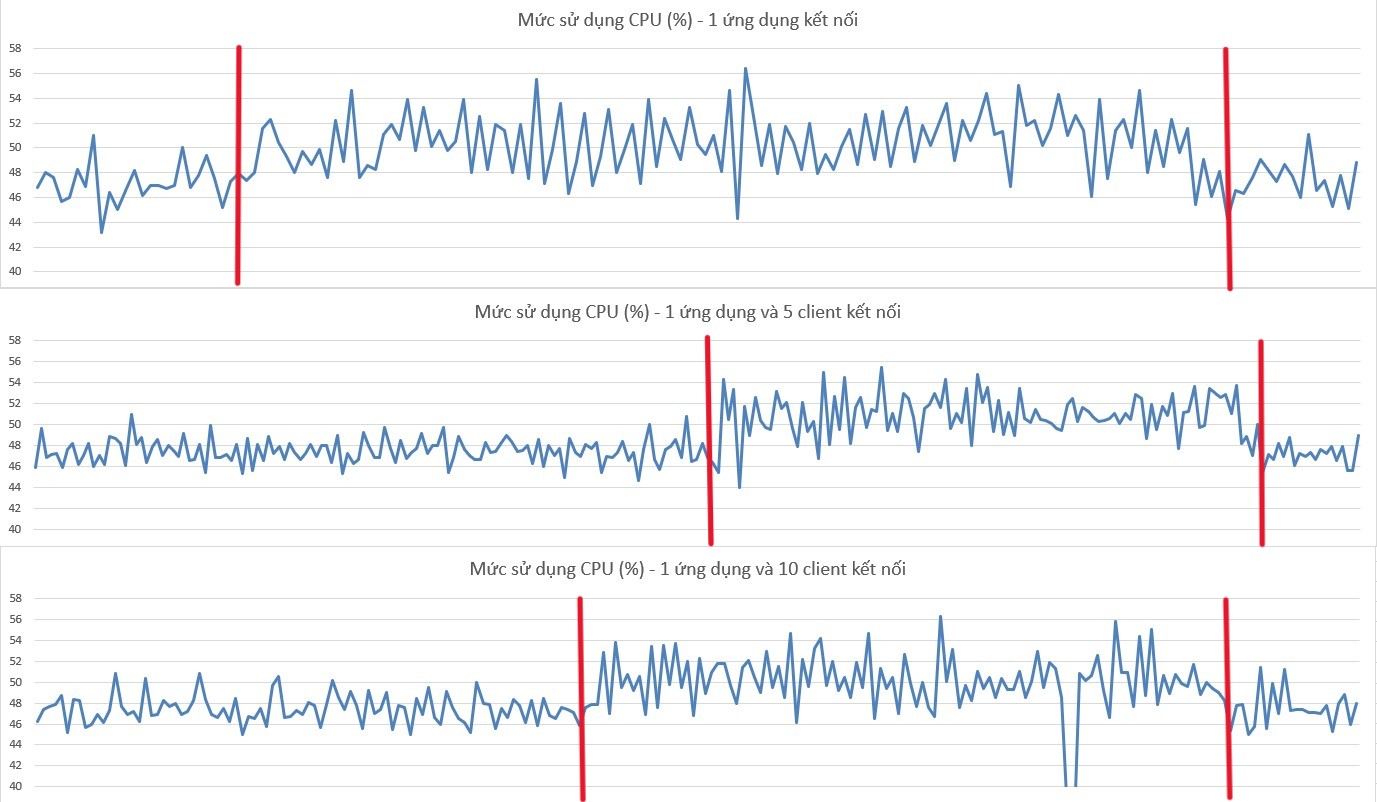
\includegraphics[width=0.9\textwidth]{Images/Result/server_cpu_2.jpg}
    \caption{Biểu đồ mức sử dụng CPU của OPC UA trên module control}
    \label{fig:server_cpu_1}
\end{figure}

Có thể thấy, do server OPC UA của module control chỉ chịu một kết nối thu thập dữ liệu của Datacenter, mức độ sử dụng CPU của server OPC UA ở mức ổn định trong khoảng từ 44\% tới 50\% trong phần đầu của biểu đồ (trước gạch kẻ màu đỏ). Khi thực hiện điều khiển 100 lần (trong phần kẻ màu đỏ), ta nhận thấy mức độ sử dụng CPU có sự gia tăng cao hơn, dao động quanh mức 50\% cho tới khi ngừng điều khiển (sau vạch kẻ màu đỏ), lượng sử dụng hạ xuống dưới 50\%. Khoảng thời gian chờ dài ở đầu biểu đồ của thí nghiệm 5 client và 10 client dùng để khởi tạo và chạy các client nhằm kết nối với Datacenter. 

Ngoài ra, trong cả ba trường hợp, lượng RAM sử dụng của chương trình không có quá nhiều thay đổi. Trong điều kiện đầu tiên, server OPC sử dụng 106.6406 MB RAM, điều kiện 5 client sử dụng 107.0312 MB RAM và 10 client sử dụng 107.0351 MB RAM. Lượng RAM gần như cố định - không bị ảnh hưởng trong suốt quá trình thực hiện điều khiển trong cả ba điều kiện thí nghiệm.

\subsubsection{Đánh giá Module Datacenter}

Datacenter là module chịu ảnh hưởng nhiều trong thí nghiệm này, bởi có nhiều client kết nối vào module này để thu thập dữ liệu nhằm mô phỏng khả năng chịu tải kết nối của hệ thống khi nhiều thiết bị người dùng kết nối vào Datacenter. Biểu đồ mức sử dụng CPU của Datacenter chạy trên Raspberry Pi 4 4GB như sau:

\begin{figure}[H]
    \centering
    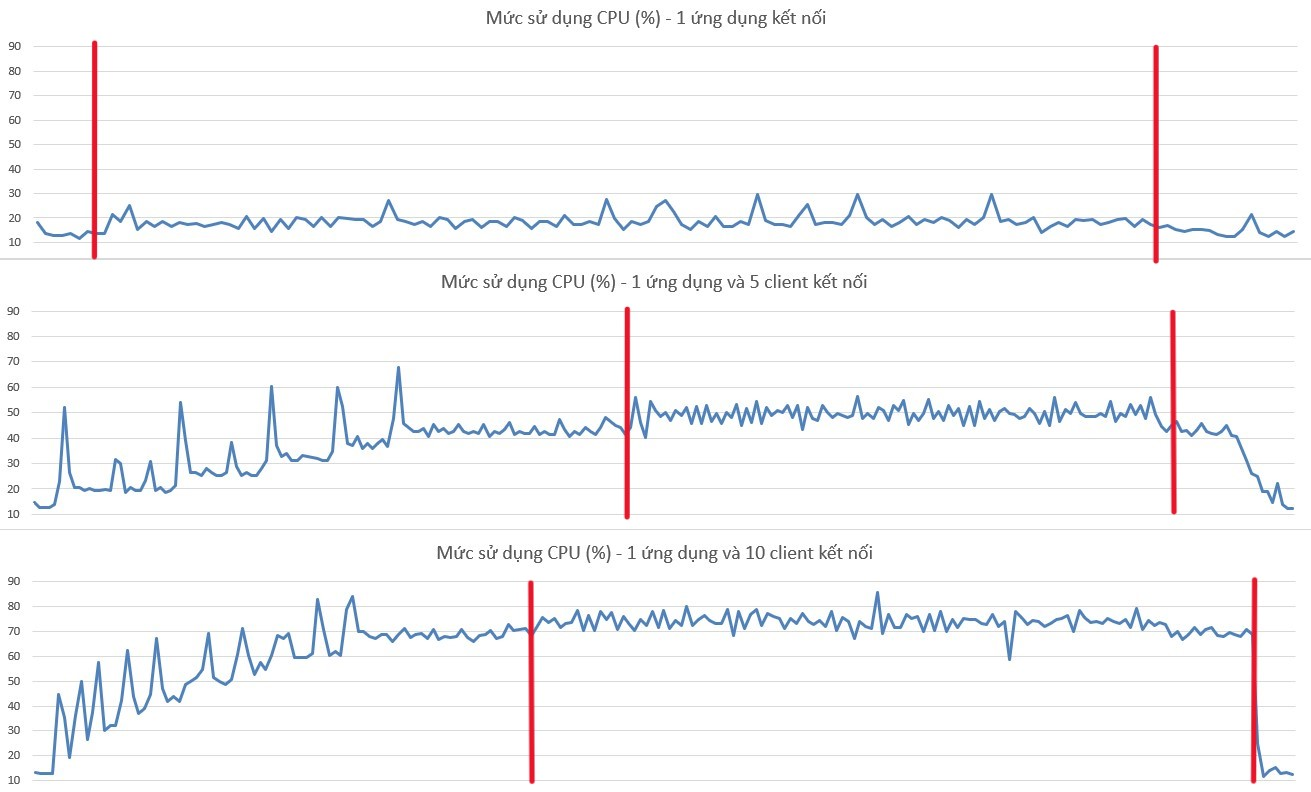
\includegraphics[width=0.9\textwidth]{Images/Result/Datacenter_cpu_2.jpg}
    \caption{Biểu đồ mức sử dụng CPU của module Datacenter}
    \label{fig:Datacenter_cpu_1}
\end{figure}

Ở biểu đồ đầu tiên, trạng thái mặc định thì lượng CPU sử dụng của Datacenter rơi vào khoảng 12\% tới 14\%. Khi có kết nối từ ứng dụng, ta nhận thấy một mũi nhọn (spike) lên tới 24\% của đồ thị thể hiện sự gia tăng đột biến về lượng CPU sử dụng trong thời gian ngắn, khi này Datacenter đang thiết lập kết nối OPC UA với ứng dụng. Sau khi kết nối hoàn tất, lượng CPU sử dụng hạ xuống và dao động quanh mức 18\%  (trong phần kẻ màu đỏ) cho tới khi ứng dụng ngắt kết nối và lượng CPU hạ xuống mức 14\%. 

Ở biểu đồ thứ hai, trong điều kiện có 5 client kết nối, ta thấy rõ được 5 spike của mức sử dụng CPU tương ứng với việc khởi tạo lần lượt 5 client kết nối vào Datacenter. Sau mỗi lần tạo kết nối, lượng CPU sử dụng bởi module Datacenter sẽ lại tăng thêm một chút: Sau client 1, tăng từ khoảng 12\% lên 20\%, sau client 2 tăng từ 20\% lên khoảng 28\%... Khi có 5 client kết nối vào Datacenter, lượng CPU sử dụng dao động quanh 41\%. Sau đó, ứng dụng kết nối vào Datacenter và thực hiện 100 lần điều khiển, lượng CPU tăng và dao động quanh 50\%, cho tới khi ứng dụng ngắt kết nối làm mức độ sử dụng rơi xuống 41\% và xuống hẳn xuống mức 10\% khi các client còn lại lần lượt ngắt kết nối.

Tương tự, với biểu đồ trong điều kiện có 10 client kết nối, ta thấy rõ 10 spike và lượng CPU sử dụng tăng đến 70\%. Khi ứng dụng kết nối và thực hiện điều khiển, lượng CPU này dao động quanh 75\% cho tới khi ngắt kết nối và tắt một lúc 10 client, khiến cho lượng sử dụng CPU xuống mức 12\% nhanh chóng.

Theo quan sát của nhóm, chương trình OPC UA trên Datacenter có sự gia tăng về lượng RAM sử dụng khi có nhiều client kết nối, từ 73.1992 MB khi chưa có client nào lên tới 111.6132 với 10 client. Tuy nhiên, lượng RAM sử dụng không hề giảm xuống khi client ngắt kết nối mà giữ nguyên, tăng một ít nếu có thêm client kết nối nhưng không vượt quá lượng client tối đa đã kết nối tới Datacenter, ngược lại, nếu vượt quá lượng client tối đa đã kết nối trước đó, lượng RAM sử dụng sẽ tăng nhiều hơn.

Theo những kết quả đo đạc được, có thể thấy kiến trúc hiện tại sẽ giới hạn các kết nối OPC UA client-server trực tiếp tới Datacenter, bởi khi có 11 client kết nối tới Datacenter, module này đã sử dụng tới 75\% CPU, và con số này sẽ tăng cao tỉ lệ thuận với số lượng client, có khả năng sẽ ảnh hưởng nặng tới hiệu năng khi module này sử dụng mức CPU nhiều hơn. Nhóm có thực hiện thử nghiệm và nhận thấy, số lượng client có thể kết nối tối đa tới Datacenter là 17 client - lúc này chương trình Datacenter sẽ chiếm đến 100\% CPU trên 1 core. Ngoài ra, module này thiếu khả năng dọn rác, nên mức tiêu thụ RAM có thể sẽ tăng lên cao nếu các client kết nối vào liên tục và sử dụng trong thời gian dài.

Để có thể áp dụng điều khiển trong thực tế, nhóm nghĩ sử dụng Raspberry Pi có thể không phù hợp, nhất là khi số lượng thiết bị cần kết nối tới tăng cao. Tùy theo nhu cầu sử dụng, ta có thể cân nhắc sử dụng các máy server cấu hình cao để tăng khả năng chịu tải tốt hơn.

\subsubsection{Đánh giá ứng dụng VR}

Ứng dụng VR giúp người dùng tiến vào không gian thực tế ảo và điều khiển thiết bị, đem lại cảm giác chân thực hơn. Đối với ứng dụng VR chạy trên kính thực tế ảo, nhóm chú ý đến ba thông số lần lượt là:
\begin{itemize}
    \item Mức sử dụng CPU - dùng để thực hiện các công việc xử lý, trao đổi dữ liệu, thu thập dữ liệu từ Datacenter thông qua OPC UA
    \item Mức sử dụng GPU - dùng cho các thao tác kết xuất khung ảnh (render) mà người dùng nhìn thấy trong ứng dụng
    \item Khung ảnh trung bình trên giây (Average Frame per second - Average fps) - Xác định số khung ảnh trung bình mà thiết bị Oculus có thể render trong ứng dụng. Fps cao và ổn định sẽ đem lại trải nghiệm mượt mà hơn cho người dùng.
\end{itemize}

Trong cả ba điều kiện thí nghiệm, nhóm đều đo đạc ba thông số này và thấy ba thông số đều tương tự nhau, nên nhóm sẽ chỉ trình bày thông số trong một điều kiện đo đạc. Biểu đồ đo đạc được thể hiện như hình dưới

\begin{figure}[H]
    \centering
    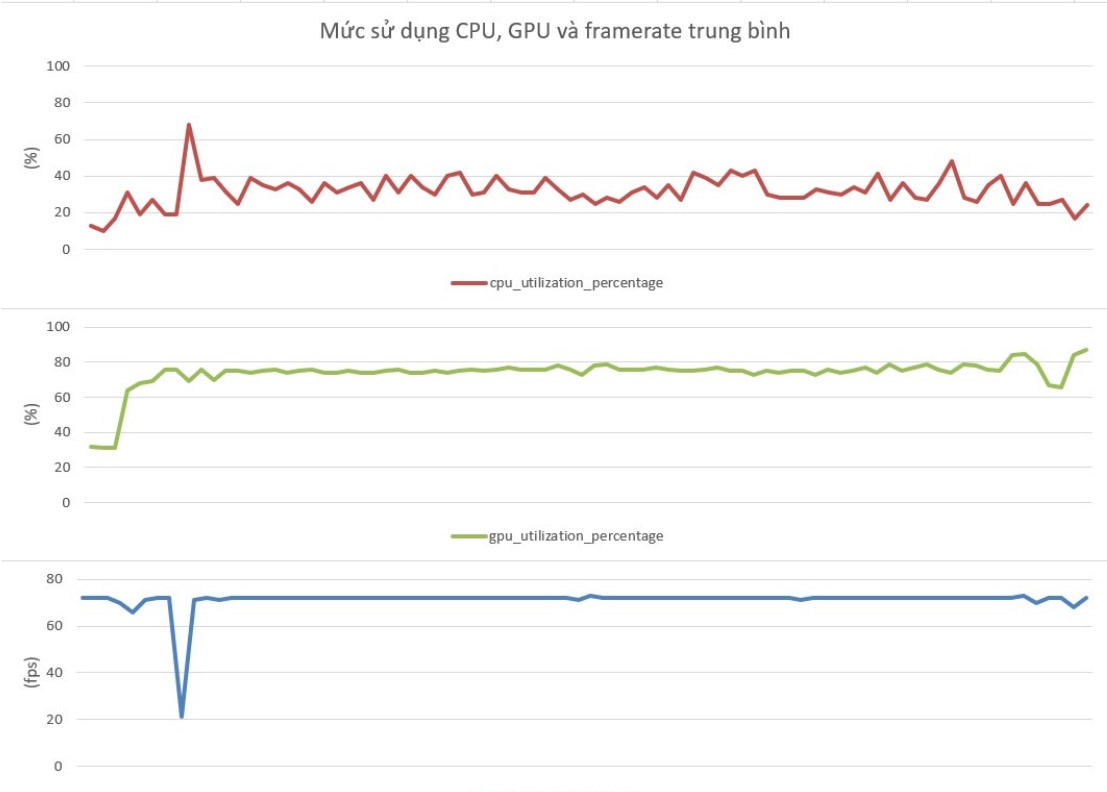
\includegraphics[width=0.9\textwidth]{Images/Result/VRapp_metrics.jpg}
    \caption{Biểu đồ mức sử dụng CPU, GPU và fps trung bình}
    \label{fig:VRapp_metrics}
\end{figure}

Trong biểu đồ, ta thấy khi ứng dụng tiến hành kết nối với Datacenter, mức sử dụng CPU có một spike lên cao, khi này ứng dụng tận dụng sức mạnh CPU nhằm thiết lập một kết nối tới OPC UA server. Đồng thời, fps rơi mạnh từ 72 fps xuống còn 20 fps. Sau khi kết nối tạo lập thành công, mức sử dụng CPU hạ xuống và dao động quanh khoảng 30\% tới 40\%, còn mức sử dụng GPU ổn định ở mức 80\%. Tương tự, fps của ứng dụng trong thí nghiệm cũng khá ổn định, dao động từ 70fps tới 72fps, gần như ít bị ảnh hưởng trong quá trình ứng dụng gửi 100 lần lệnh điều khiển tới Datacenter.

Khi ngắt kết nối ứng dụng tới Datacenter, ta nhận thấy một sự tụt fps nhỏ ở cuối biểu đồ, tương đương với sự hạ thấp mức sử dụng GPU và một spike nhỏ của mức dùng CPU sau đó.

Ứng dụng VR có sự giảm fps mạnh khi tạo kết nối với Datacenter và một ít khi ngắt kết nối. Ngoài ra, trong quá trình sử dụng, nếu chỉ gọi các giao thức điều khiển đơn giản, ứng dụng chạy mượt với lượng fps ổn định khoảng 70 fps. Khi chạy các chức năng phức tạp hơn, fps của ứng dụng có giảm nhiều hơn, nhưng vẫn đảm bảo cao hơn 60fps trong suốt quá trình hoạt động. Theo góp ý của thầy phản biện, nhóm đã thực hiện một số tối ưu tốt về mặt đồ họa, từ ứng dụng ngốn 100\% GPU và mức fps dao động mạnh, đã giảm xuống 80\% GPU và mức fps cao, ổn định 72 trong quá trình sử dụng ứng dụng, đảm bảo khả năng mở rộng, gia tăng số lượng vật thể, tương tác trong tương lai.

\subsubsection{Đánh giá thời gian trễ trọn vòng (RTT)}

Thời gian trễ trọn vòng (Round Trip Time - RTT) là thời gian được đo bằng đơn vị mili giây được tính từ lúc một yêu cầu mạng đi từ điểm xuất phát đến điểm đến và quay trở lại nơi bắt đầu. Trong thí nghiệm này, nhóm thực hiện đo RTT bằng cách gửi yêu cầu điều khiển từ ứng dụng và đo thời gian cho tới khi nhận lại được phản hồi tới ứng dụng. RTT được đo trong cả ba điều kiện: chỉ một ứng dụng kết nối, 5 client và ứng dụng kết nối, 10 client và ứng dụng kết nối. 

\begin{longtblr}[
caption = {Kết quả đo RTT trong thí nghiệm},
label = {tblr:my-table},
entry = {Kết quả đo RTT trong thí nghiệm}
]{
hlines,vlines,
colspec = {X[2,c]X[2,c]X[2,c]X[2,c]},
columns = {valign = m},
}
 & \textbf{1 app} & \textbf{5 client, 1 app} & \textbf{10 client, 1 app} \\
\textbf{Trung bình  }        & 38.9837 & 46.7935 & 65.0815 \\
\textbf{Trung vị  }          & 27.319 & 31.303 & 40.265 \\
\textbf{Độ lệch chuẩn }      & 45.4120 & 60.8002 & 133.0796 \\
\textbf{Độ lệch}             & 4.7776 & 4.4399 & 7.4434 \\
\textbf{Tối thiểu }          & 12.145 & 13.121 & 12.572 \\
\textbf{Tối đa}              & 350.994 & 457.452 & 1230.646 \\
\end{longtblr}

\begin{figure}[H]
    \centering
    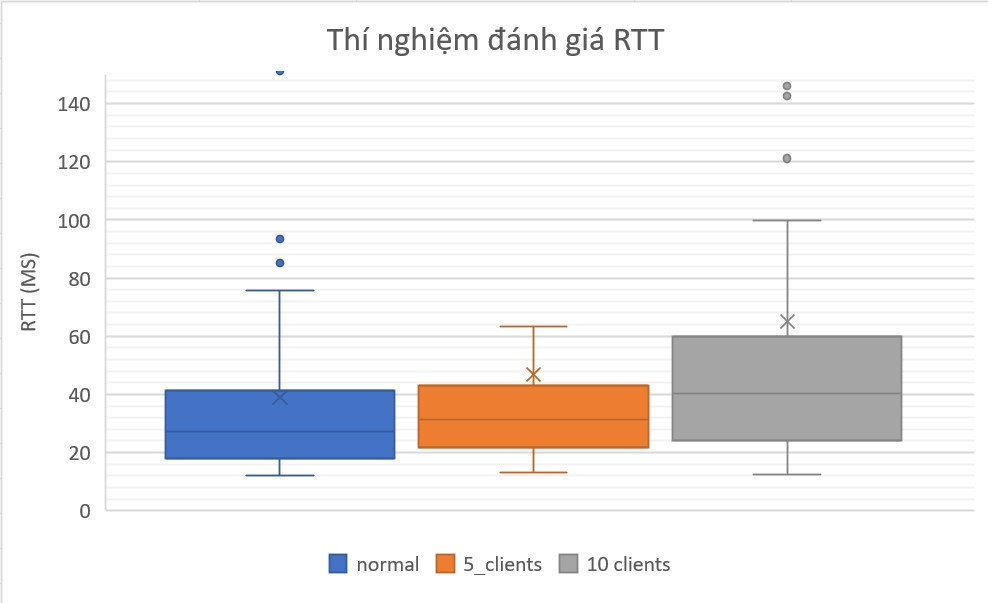
\includegraphics[width=0.9\textwidth]{Images/Result/rtt_exp.jpg}
    \caption{Biểu đồ Box-plot RTT trong thí nghiệm đã lược bỏ một số outliner}
    \label{fig:rtt_exp}
\end{figure}

Quan sát kết quả trong bảng và biểu đồ box-plot, nhóm có nhận xét là RTT có xu hướng tăng lên khi số lượng client kết nối vào Datacenter càng nhiều. Trung bình RTT trong ba điều kiện lần lượt là 38.9837ms, 46.7935ms và 65.0815ms. Dù trung bình khá cao, tuy nhiên các con số này không phản ánh được RTT chung trong các thí nghiệm do dữ liệu bị lệch phải (right-skew) ở cả ba thí nghiệm. Ta có thể nhận thấy điều này qua giá trị độ lệch dương, và giá trị trung bình lớn hơn giá trị trung vị. Điều này có nghĩa rằng độ lớn giá trị RTT trong thí nghiệm tập trung nhiều ở phía trái, tức có nhiều giá trị RTT nhỏ so với các giá trị RTT lớn. Nhóm cũng nhận thấy qua biểu đồ box-plot một lượng lớn điểm dữ liệu bé hơn giá trị trung bình ở cả ba điều kiện thí nghiệm.

Độ lệch chuẩn có xu hướng tăng lên khi số lượng client kết nối vào Datacenter tăng lên, chứng tỏ sự bất ổn định của khả năng phản hồi của Datacenter khi số lượng client kết nối vào tăng cao. Ngoài ra, nhóm cũng nhận xét giá trị tối thiểu - tối đa trong ba điều kiện thí nghiệm: trong điều kiện chỉ có một ứng dụng, RTT tốt nhất là 12.145ms, còn lớn nhất là 350.994ms; khi có 5 client và ứng dụng kết nối, RTT tốt nhất là 13.121ms, giá trị lớn nhất cao hơn là 457.452ms; khi tăng lên tới 10 client và ứng dụng, RTT tốt nhất là 12.572ms, và tệ nhất là 1230.646ms. 

Giải thích cho việc ứng dụng có RTT cao, từ 12ms trở lên, nhóm cho rằng có nhiều nguyên nhân: 

\begin{itemize}
    \item Thời gian mã hóa và giải mã gói tin OPC UA diễn ra ở module Control, module Datacenter và ứng dụng VR.
    \item Cách hiện thực chương trình trên module Datacenter và module Control chưa được tối ưu, khiến các request bị chậm trễ.
    \item Ảnh hưởng của điều kiện mạng, nhiễu sóng hay số lượng truy cập cao.
\end{itemize}




\subsection{Đánh giá độ chính xác của chức năng phân loại rác}

Để có thể đánh giá được mức độ chính xác của chức năng phân loại rác bán tự động, nhóm đã tiến hành một số thí nghiệm với hai mục tiêu sau:
\begin{itemize}
    \item Kiểm tra khả năng nhận diện rác của camera tích hợp trên cánh tay robot.
    \item Kiểm tra tính hiệu quả của chức năng phân loại - khả năng hút và thả chính xác.
\end{itemize}

\subsubsection{Khả năng nhận diện}
Ở thí nghiệm này, nhóm tiến hành cho camera nhận diện lần lượt từng thẻ rác. Thẻ rác cần nhận diện sẽ được đặt chung với tất cả các thẻ rác còn lại và được sắp xếp một cách ngẫu nhiên trước camera. Mỗi thẻ rác sẽ được nhận diện 20 lần và với mỗi lần nhận diện thì các thẻ rác sẽ được thay đổi lại vị trí khác nhau, từ đó nhóm sẽ ghi nhận lại số lần nhận diện đúng cũng như số lần nhận diện sai. Và để có được đánh giá khách quan dựa trên số liệu đo đạc được thì nhóm sẽ áp dụng một số thước đo mô hình phân loại như thước đo đánh giá Độ chính xác (Accuracy), Độ chuẩn xác (Precision) và Độ phủ (Recall) để tính toán phần trăm nhận diện chính xác của camera. Trước hết, chúng tôi sẽ giới thiệu đôi nét về các thước đo mô hình phân loại này.

Giả sử chúng ta đang có một mô hình phân loại rác và mong muốn của chúng ta là nhận diện được một thẻ rác (BAD) so với tất cả các thẻ rác còn lại (GOOD). Kích thước của tập dữ liệu sẽ là 9 thẻ GOOD và 1 thẻ BAD.
Để thuận tiện cho việc diễn giải thì nhãn BAD tương ứng với giá trị 1 được gọi là dương tính (positive) và nhãn GOOD tương ứng với giá trị 0 được gọi là âm tính (negative). Và để làm cơ sở cho những thước đo quan trọng đối với bài toán phân loại thì chúng ta sẽ sử dụng những chỉ số sau:
\begin{itemize}
    \item \textbf{TP (True Positive)}: Tổng số trường hợp dự báo khớp mẫu dương tính.
    \item \textbf{TN (True Negative)}: Tổng số trường hợp dự báo khớp mẫu âm tính.
    \item \textbf{FP (False Positive)}: Tổng số trường hợp dự báo các quan sát thuộc nhãn âm tính thành dương tính.
    \item \textbf{FN (False Negative)}: Tổng số trường hợp dự báo các quan sát thuộc nhãn dương tính thành âm tính.
\end{itemize}

Khi xây dựng mô hình phân loại chúng ta sẽ muốn biết một cách khái quát tỷ lệ các trường hợp được dự báo đúng trên tổng số các trường hợp là bao nhiêu. Tỷ lệ đó được gọi là \textbf{\textit{Độ chính xác (Accuracy)}}. Độ chính xác giúp ta đánh giá hiệu quả dự báo của mô hình trên một bộ dữ liệu. Độ chính xác càng cao thì mô hình của chúng ta càng tốt. Độ chính xác được tính bằng tổng số trường hợp dự báo đúng trên cả âm tính và dương tính chia cho tổng số mẫu:
\begin{equation}
    Accuracy = \frac{TP + TN}{TP + TN + FP + FN}
\end{equation}

\textbf{\textit{Độ chuẩn xác (Precision)}} trả lời cho câu hỏi trong các trường hợp được dự báo là dương tính thì có bao nhiêu trường hợp là đúng ? Và tất nhiên độ chuẩn xác càng cao thì mô hình của chúng ta càng tốt trong việc phân loại hồ sơ BAD. Công thức của độ chuẩn xác được tính trên nhóm dương tính như sau:
\begin{equation}
    Precision = \frac{TP}{TP + FP}
\end{equation}

Cũng có ý nghĩa gần tương tự như độ chuẩn xác, có cùng tử số nhưng có một chút khác biệt về mẫu số trong công thức tính toán, và cũng là một chỉ số giúp đo lường hiệu suất dự báo trên nhóm dương tính, đó là \textbf{\textit{Độ phủ (Recall)}}. 
Độ phủ đo lường tỷ lệ dự báo chính xác các trường hợp dương tính trên toàn bộ các mẫu thuộc nhóm dương tính. Công thức của recall như sau:
\begin{equation}
    Recall = \frac{TP}{TP + FN}
\end{equation}

Tuy nhiên, hạn chế của Thước đo Độ chính xác là chỉ đo lường trên tất cả các nhãn mà không quan tâm đến từng nhãn. Do đó nó không phù hợp để đánh giá những tác vụ mà tầm quan trọng của việc dự báo các nhãn không còn như nhau. Hay cụ thể hơn, trong bài toán của chúng ta, việc chúng ta phát hiện đúng thẻ rác mong muốn (thẻ BAD) quan trọng hơn việc chúng ta phát hiện đúng các thẻ rác khác (các thẻ GOOD). Vì vậy, đối với thí nghiệm này chúng ta sẽ quan tâm hơn tới độ chính xác nhưng được đo lường chỉ trên nhãn BAD hơn và những thước đo như Độ chuẩn xác (precision), Độ phủ (recall) sẽ giúp chúng ta đánh giá chuyên biệt trên nhóm này thay vì Độ chính xác. 

Vì vậy, sau khi tiến hành đo đạc với 12 thẻ rác khác nhau, chúng tôi thu được kết quả như sau:



\begin{longtblr}[
caption = {Kết quả nhận diện của camera đối với 12 thẻ rác},
label = {tblr:ai_label_precision},
entry = {Kết quả nhận diện của camera đối với 12 thẻ rác}
]{
hlines,vlines,
colspec = {X[2,c]X[2,c]X[2,c]X[2,c]},
columns = {valign = m},
}
\textbf{Thẻ rác} & \textbf{Precision} & \textbf{Recall} & \textbf{f1 score} \\
\textbf{Banana Peel  }        & 1 & 1 & 1 \\
\textbf{Broken Bones  }          & 1 & 0.35 & 0.518 \\
\textbf{Ketchup }      & 1 & 0.95 & 0.974 \\
\textbf{Marker}             & 1 & 0.65 & 0.78 \\
\textbf{Oral Liquid Bottle }          & 1 & 0.85 & 0.918 \\
\textbf{Storage Battery}              & 1 & 0.75 & 0.857 \\
\textbf{Plastic Bottle  }        & 1 & 0.95 & 0.974 \\
\textbf{Toothbrush  }          & 1 & 0.5 & 0.667 \\
\textbf{Umbrella }      & 1 & 0.5 & 0.667 \\
\textbf{Plate}             & 1 & 0.95 & 0.974 \\
\textbf{Cigarette End }          & 1 & 0.7 & 0.824 \\
\textbf{Disposable Chopsticks}              & 1 & 0.35 & 0.518 \\
\end{longtblr}

Qua kết quả trên ta có thể thấy độ chuẩn xác (precision) của tất cả các thẻ đều là 1. Điều này có nghĩa là khi có một thẻ được nhận diện là BAD thì khả năng rất cao thẻ đó đúng là BAD bởi xác suất 100\% là một mức tin cậy rất cao. 

Về độ phủ thì ta có thể thấy Banana Peel là thẻ cho kết quả cao nhất (100\%) và điều này có nghĩa là 100\% những thẻ Banana Peel đều được nhận diện đúng là Banana Peel. Bên cạnh đó, những thẻ như Ketchup, Plastic Bottle và Plate cũng có kết quả tương đối cao (95\%). Ngược lại, Broken Bones là thẻ có kết quả nhận diện kém nhất trong các thẻ (35\% - có nghĩa trong tất cả các thẻ Broken Bones thì chỉ có 35\% số thẻ được nhận diện đúng). Và lý do của sự chênh lệch tỉ lệ nhận diện của các thẻ nhìn chung đến từ ánh sáng, màu sắc và hình vẽ trên thẻ (thẻ có màu sắc tươi tắn, hình vẽ trên thẻ to, rõ thì tỉ lệ nhận diện cao hơn; ngược lại, thẻ có màu sắc nhạt nhòa, hình vẽ nhỏ, rời rạc thì sẽ có tỉ lệ nhận diện thấp hơn).

Ngoài ra, dựa trên độ chuẩn xác và độ phủ thì chúng tôi còn tính toán thêm chỉ số f1 score - trung bình điều hòa giữa độ chuẩn xác và độ phủ. Đây là thước đo kết hợp cả hai chỉ số trên nhằm có được đánh giá khách quan hơn so với việc quá lạc quan vào mô hình khi chỉ nhìn vào độ chuẩn xác hoặc quá bi quan nếu chỉ dựa vào độ phủ. 
Và ta có thể quan sát thấy chỉ số f1 của tất cả các thẻ đều lớn hơn 50\%, đây chính là tỉ lệ dự báo đúng của các trường hợp mẫu dương tính. Qua đó, có thể thấy đây là một mô hình có sức mạnh ở mức trung bình.

\subsubsection{Khả năng hút-thả rác hiệu quả}
Ở thí nghiệm này, các thẻ rác sẽ được sắp xếp một cách ngẫu nhiên trước cánh tay. Và cánh tay sẽ được điều khiển hút-thả một cách bán tự động để phân loại tất cả các thẻ rác vào thùng rác.
Thí nghiệm sẽ được thực hiện 100 lần và chúng tôi sẽ ghi nhận lại số lần hút/ thả chính xác cũng như không chính xác. Và kết quả thí nghiệm thu được như sau:

\newpage
\begin{longtblr}[
caption = {Kết quả đo khả năng hút-thả rác},
label = {tblr:suck_release_precision},
entry = {Kết quả đo khả năng hút-thả rác}
]{
hlines,vlines,
colspec = {X[2,c]X[2,c]X[2,c]X[2,c]},
columns = {valign = m},
}
 & \textbf{Hút} & \textbf{Thả}\\
\textbf{Số lần chính xác  }        & 91 & 72\\
\textbf{Tỉ lệ chính xác  }          & 0.91 & 0.72\\
\end{longtblr}

\begin{figure}[H]
    \centering
    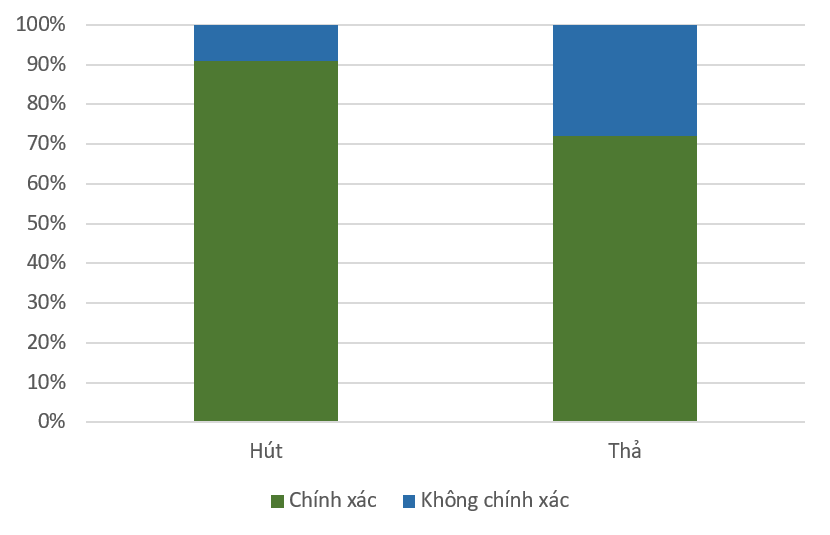
\includegraphics[width=0.9\textwidth]{Images/Result/hut_tha.png}
    \caption{Kết quả đo khả năng hút-thả rác}
    \label{fig:hut_tha}
\end{figure}

Sau nhiều lần thí nghiệm thì ta có thể thấy tỉ lệ hút chính xác rác khá cao, chiếm 91\% và tỉ lệ thả đúng vào thùng rác cũng tương đối, chiếm 72\%. Các yếu tố như ánh sáng môi trường, chất lượng camera, vị trí vật thể cũng là nguyên nhân lớn dẫn đến việc nhận diện và hút/thả không chính xác. Tuy nhiên, tỉ lệ chính xác này cũng tương đối cao, từ đó có thể thấy được mức độ hoạt động của cánh tay tương đối hiệu quả và ổn định đối với chức năng hút-thả rác bán tự động.
